\documentclass{beamer}

\usepackage{appendixnumberbeamer}
\usepackage[USenglish]{babel}
\usepackage[backend=bibtex,citestyle=authortitle]{biblatex}
\usepackage[scale=2]{ccicons}
\usepackage{graphicx}
\usepackage{listings}
\usepackage{tikz}

% this actually isn't totally hideous:
\usetheme[numbering=counter, progressbar=frametitle, sectionpage=none]{metropolis}
\setbeamertemplate{bibliography item}[text]
\setbeamertemplate{frametitle continuation}{}

\graphicspath{{../figures/}}

\title{Composable Concurrency Models}
\date{November 19, 2016}
\author{Dan Stelljes}

\bibliography{references}

\AtEveryBibitem{\clearfield{note}}
\AtEveryBibitem{\clearfield{url}}

\begin{document}
  \maketitle

  \section{Introduction}

  \begin{frame}
    \centering
    \resizebox{\linewidth}{!}{\begin{tikzpicture}
  \onslide<1->{
    \node at (0,0) {
      
\includegraphics[width=300pt]{browser}
    };
  }

  \onslide<2>{
    \path (-2.25,2.75) [draw=none, fill=darkgray, opacity=0.75] ellipse (60pt and 25pt);
    \node [text=white] at (-2.25,2.75) {
      Multiple tabs
    };

    \draw (2.25,2.25) [draw=none, fill=darkgray, opacity=0.75] ellipse (60pt and 25pt);
    \node [text=white] at (2.25,2.25) {
      Suggestions
    };

    \draw (0,0.5) [draw=none, fill=darkgray, opacity=0.75] ellipse (60pt and 25pt);
    \node [text=white] at (0,0.5) {
      Page rendering
    };

    \draw (-3,-1.5) [draw=none, fill=darkgray, opacity=0.75] ellipse (60pt and 25pt);
    \node [text=white] at (-3,-1.5) {
      Event handling
    };

    \draw (2.5,-1.5) [draw=none, fill=darkgray, opacity=0.75] ellipse (60pt and 25pt);
    \node [text=white] at (2.5,-1.5) {
      Background processes
    };
  }

  \onslide<3>{
    \node at (0,-0.62) {
      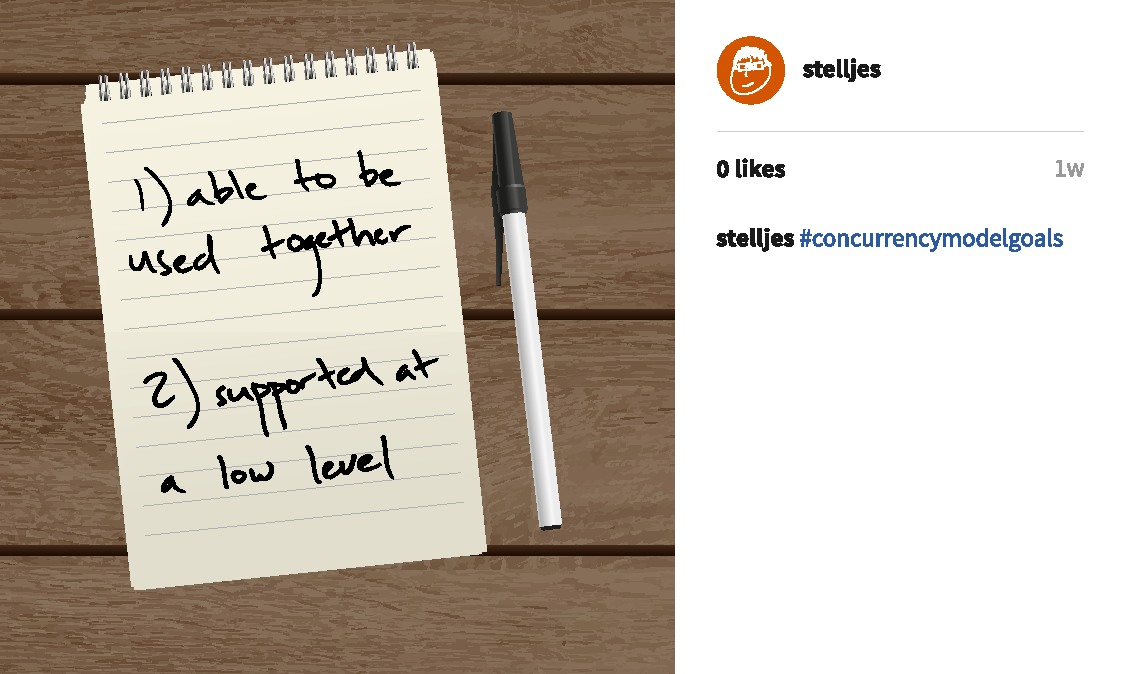
\includegraphics[width=220pt]{goals}
    };
  }
\end{tikzpicture}
}
  \end{frame}

  \section{Background}

  \subsection{Concurrency}

  \begin{frame}
    \frametitle{Concurrency}

    \textbf{The ``happens before'' ($\rightarrow$) relation~\footcite{Lamport1977}}

    $A \rightarrow B$ if one of the following is true:

    \begin{enumerate}
      \item $A$ and $B$ are operations in the same thread and $A$ occurs before $B$.
      \item $A$ is the sending of a message by one thread and $B$ is the receipt of the same message by another thread.
    \end{enumerate}

    If $A \rightarrow B$ and $B \rightarrow C$, then $A \rightarrow C$.

    $A$ and $B$ are said to be concurrent if $A \nrightarrow B$ and $B \nrightarrow A$.
  \end{frame}

  \subsection{Complications}

  \begin{frame}
    \frametitle{Complications}

    \begin{itemize}
      \item \textbf{Sequential program:} Does the order of operations yield a correct result?
      \vfill
      \item \textbf{Concurrent program:} Does \emph{every possible} order of operations yield a correct result?
    \end{itemize}
  \end{frame}

  \begin{frame}
    \frametitle{Complications}
    \centering

    \textbf{Single thread:}
    \vfill
    \resizebox{0.9\linewidth}{!}{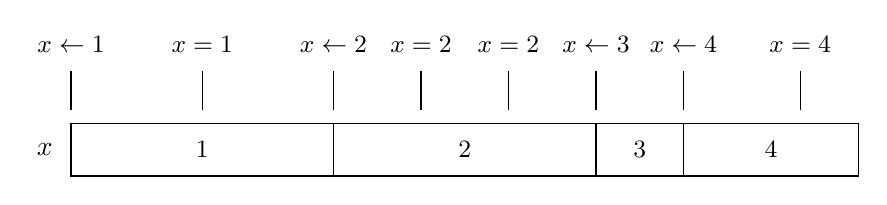
\begin{tikzpicture}
  \node at (-5.333,0) { $x$ };

  \draw (-5,-0.333) rectangle (-1.667,0.333) node [midway] { \small $1$ };
  \draw (-1.667,-0.333) rectangle (1.667,0.333) node [midway] { \small $2$ };
  \draw (1.667,-0.333) rectangle (2.778,0.333) node [midway] { \small $3$ };
  \draw (2.778,-0.333) rectangle (5,0.333) node [midway] { \small $4$ };

  \draw (-5,0.5) -- (-5,1) node [above=3pt] { \small $x \leftarrow 1$ };
  \draw (-3.333,0.5) -- (-3.333,1) node [above=3pt] { \small $x = 1$ };

  \draw (-1.667,0.5) -- (-1.667,1) node [above=3pt] { \small $x \leftarrow 2$ };
  \draw (-0.555,0.5) -- (-0.555,1) node [above=3pt] { \small $x = 2$ };
  \draw (0.555,0.5) -- (0.555,1) node [above=3pt] { \small $x = 2$ };

  \draw (1.667,0.5) -- (1.667,1) node [above=3pt] { \small $x \leftarrow 3$ };

  \draw (2.778,0.5) -- (2.778,1) node [above=3pt] { \small $x \leftarrow 4$ };
  \draw (4.26,0.5) -- (4.26,1) node [above=3pt] { \small $x = 4$ };
\end{tikzpicture}
}
  \end{frame}

  \begin{frame}
    \frametitle{Complications}
    \centering

    \textbf{Multiple threads:}
    \vfill
    \resizebox{0.9\linewidth}{!}{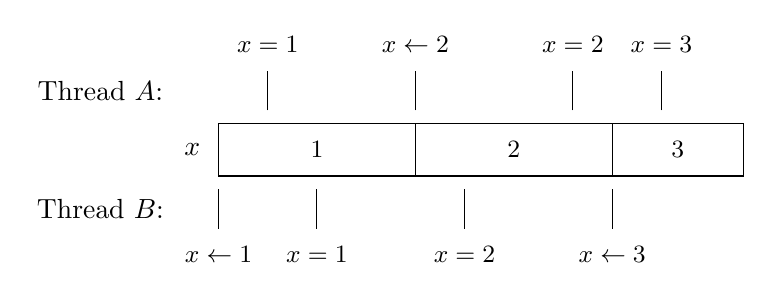
\begin{tikzpicture}
  \node at (-6.5,0.75) { Thread $A$: };
  \node at (-6.5,-0.75) { Thread $B$: };
  \node at (-5.333,0) { $x$ };

  \draw (-5,-0.333) rectangle (-2.5,0.333) node [midway] { \small $1$ };
  \draw (-2.5,-0.333) rectangle (0,0.333) node [midway] { \small $2$ };
  \draw (0,-0.333) rectangle (1.667,0.333) node [midway] { \small $3$ };

  \draw (-5,-0.5) -- (-5,-1) node [below=3pt] { \small $x \leftarrow 1$ };
  \draw (-4.375,0.5) -- (-4.375,1) node [above=3pt] { \small $x = 1$ };
  \draw (-3.75,-0.5) -- (-3.75,-1) node [below=3pt] { \small $x = 1$ };

  \draw (-2.5,0.5) -- (-2.5,1) node [above=3pt] { \small $x \leftarrow 2$ };
  \draw (-1.875,-0.5) -- (-1.875,-1) node [below=3pt] { \small $x = 2$ };
  \draw (-0.5,0.5) -- (-0.5,1) node [above=3pt] { \small $x = 2$ };

  \draw (0,-0.5) -- (0,-1) node [below=3pt] { \small $x \leftarrow 3$ };
  \draw (0.625,0.5) -- (0.625,1) node [above=3pt] { \small $x = 3$ };
\end{tikzpicture}
}
  \end{frame}

  \begin{frame}
    \frametitle{Complications}

    \centering
    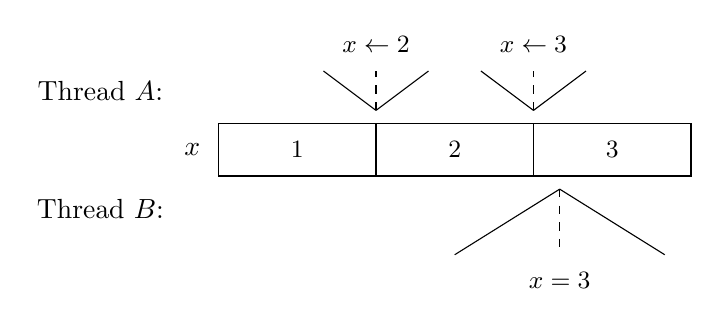
\begin{tikzpicture}
  \node at (-4.5,0.75) { Thread $A$: };
  \node at (-4.5,-0.75) { Thread $B$: };
  \node at (-3.333,0) { $x$ };

  \draw (-3,-0.333) rectangle (-1,0.333) node [midway] { \small $1$ };
  \draw (-1,-0.333) rectangle (1,0.333) node [midway] { \small $2$ };
  \draw (1,-0.333) rectangle (3,0.333) node [midway] { \small $3$ };

  \draw (-1.667,1) -- (-1,0.5) (-1,0.5) -- (-0.333,1);
  \draw [dashed] (-1,0.5) -- (-1,1) node [above=3pt] { \small $x \leftarrow 2$ };

  \draw (0.333,1) -- (1,0.5) (1,0.5) -- (1.667,1);
  \draw [dashed] (1,0.5) -- (1,1) node [above=3pt] { \small $x \leftarrow 3$ };

  \draw (0,-1.333) -- (1.333,-0.5) (1.333,-0.5) -- (2.667,-1.333);
  \draw [dashed] (1.333,-0.5) -- (1.333,-1.333) node [below=3pt] { \small $x = 3$ };
\end{tikzpicture}

  \end{frame}

  \subsection{Consistency models}

  \begin{frame}
    \frametitle{Linearizability}

    \begin{figure}
      \centering
      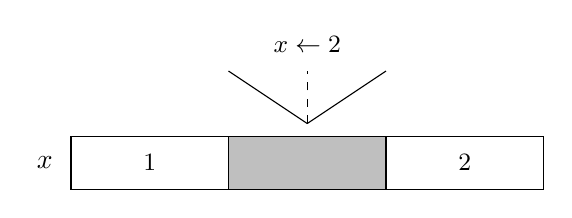
\begin{tikzpicture}
  \node at (-3.333,0) { $x$ };

  \draw (-3,-0.333) rectangle (-1,0.333) node [midway] { \small $1$ };
  \draw [fill=lightgray] (-1,-0.333) rectangle (1,0.333);
  \draw (1,-0.333) rectangle (3,0.333) node [midway] { \small $2$ };

  \draw (-1,1.167) -- (0,0.5) (0,0.5) -- (1,1.167);
  \draw [dashed] (0,0.5) -- (0,1.167) node [above=3pt] { \small $x \leftarrow 2$ };
\end{tikzpicture}

    \end{figure}

    \vfill

    \begin{itemize}
      \item Linearizability guarantees that the completion of an operation on a single object will appear to be instantaneous.
      \item The results of a linearizable operation will be visible as soon as the operation is complete.
    \end{itemize}
  \end{frame}

  \begin{frame}
    \frametitle{Serializability}

    \begin{figure}
      \centering
      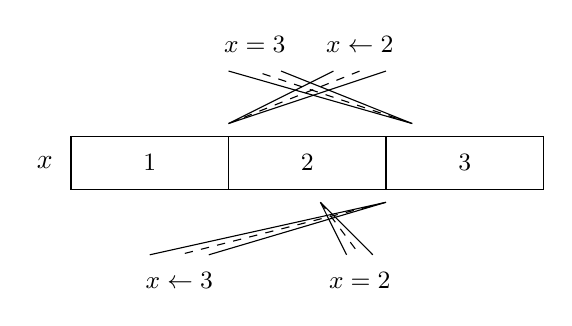
\begin{tikzpicture}
  \node at (-3.333,0) { $x$ };

  \draw (-3,-0.333) rectangle (-1,0.333) node [midway] { \small $1$ };
  \draw (-1,-0.333) rectangle (1,0.333) node [midway] { \small $2$ };
  \draw (1,-0.333) rectangle (3,0.333) node [midway] { \small $3$ };

  \draw (0.333,1.167) -- (-1,0.5) (-1,0.5) -- (1,1.167);
  \draw [dashed] (-1,0.5) -- (0.667,1.167) node [above=3pt] { \small $x \leftarrow 2$ };

  \draw (0.5,-1.167) -- (0.167,-0.5) (0.167,-0.5) -- (0.833,-1.167);
  \draw [dashed] (0.167,-0.5) -- (0.667,-1.167) node [below=3pt] { \small $x = 2$ };

  \draw (-2,-1.167) -- (1,-0.5) (1,-0.5) -- (-1.25,-1.167);
  \draw [dashed] (1,-0.5) -- (-1.625, -1.167) node [below=3pt] { \small $x \leftarrow 3$ };

  \draw (-1,1.167) -- (1.333,0.5) (1.333,0.5) -- (-0.333,1.167);
  \draw [dashed] (1.333,0.5) -- (-0.667,1.167) node [above=3pt] { \small $x = 3$ };
\end{tikzpicture}

    \end{figure}

    \vfill

    \begin{itemize}
      \item Serializability guarantees that operations can occur in any order as long as an equivalent sequential ordering exists.
      \item While a serializable set of operations is being executed, it appears to be the only set of operations being executed.
    \end{itemize}
  \end{frame}

  \begin{frame}
    \frametitle{Strict serializability}

    \begin{itemize}
      \item Linearizability is a guarantee of consistency.
      \item Serializability is a guarantee of isolation.
      \item Together, linearizability and serializability guarantee strict serializability---an ordering of operations is equivalent to some sequential ordering and that ordering corresponds to the execution ordering in real time.~\footcite{Herlihy1990}
    \end{itemize}
  \end{frame}

  \section{Common concurrency models}

  \begin{frame}
    \frametitle{Concurrency models}

    \begin{itemize}
      \item Modern languages usually support several different models.
      \item Common concurrency models fall into four general categories:~\footcite{Swalens2014}
      \begin{enumerate}
        \item Atomic variables
        \item Software transactional memory (STM)
        \item Communicating threads
        \item Proxies
      \end{enumerate}
    \end{itemize}
  \end{frame}

  \subsection{Atomic variables}

  \begin{frame}[fragile]
    \frametitle{Atomic variables}

    \begin{lstlisting}[basicstyle=\scriptsize\ttfamily,language=C]
      void unsafe_increment() {
        *variable++;
      }
    \end{lstlisting}
% "good indentation? lol get bent" —Beamer
\end{frame}

  \begin{frame}[fragile]
    \frametitle{Atomic variables}

    \begin{lstlisting}[basicstyle=\scriptsize\ttfamily,language=C]
      int fetch_and_add(int* variable, int increment) {
        // obtain exclusive control of variable

        int value = *variable + increment;
        *variable = value;

        // release exclusive control of variable

        return value;
      }

      void safe_increment() {
        fetch_and_add(variable, 1);
      }
    \end{lstlisting}
\end{frame}

  \begin{frame}[fragile]
    \frametitle{Atomic variables}

    \begin{lstlisting}[basicstyle=\scriptsize\ttfamily,language=Java]
      AtomicInteger variable = new AtomicInteger(23);
      variable.incrementAndGet();
    \end{lstlisting}

    \vfill

    \begin{lstlisting}[basicstyle=\scriptsize\ttfamily,language=Lisp]
      (def variable (atom 23))
      (swap! variable inc)
    \end{lstlisting}
\end{frame}

  \begin{frame}
    \frametitle{Atomic variables}

    Atomic variables are\ldots

    \begin{itemize}
      \item used to share objects that are shared by multiple threads but don't require coordinated updates
      \item usually implemented in hardware, guaranteeing linearizability at the lowest level possible
      \item used to implement higher-level concurrency control mechanisms and concurrent data structures
    \end{itemize}
  \end{frame}

  \subsection{Software transactional memory}

  \begin{frame}
    \frametitle{Software transactional memory}

    Another approach to working with shared memory:~\footcite{Shavit1995}

    \begin{enumerate}
      \item A thread writes to a shared memory location, keeping track of the transaction in a log.
      \item If there are conflicting changes at the end of the transaction, the transaction is aborted and retried until it eventually succeeds.
      \item Once a transaction succeeds, changes will become visible to other threads.
    \end{enumerate}
  \end{frame}

  \begin{frame}[fragile]
    \frametitle{Software transactional memory}

    \begin{lstlisting}[basicstyle=\scriptsize\ttfamily,language=Java]

      import akka.stm.*;

      Ref<Integer> reference = new Ref<Integer>(23);

      new Atomic<Integer>() {
        public Integer atomically() {
          int value = reference.get();
          reference.set(value++);

          return value;
        }
      }.execute();
    \end{lstlisting}

    \vfill

    \begin{lstlisting}[basicstyle=\scriptsize\ttfamily,language=Lisp]
      (def reference (ref 23))
      (dosync (alter reference inc))
    \end{lstlisting}
\end{frame}

  \begin{frame}
    \frametitle{Software transactional memory}

    STM is\ldots

    \begin{itemize}
      \item used to share objects that need to be accessed and modified by multiple threads
      \item a simple alternative to lock-based programming
      \item susceptible to performance decreases caused by maintaining a transaction log and retrying transactions
      \item unable to execute operations that cannot be undone or retried
    \end{itemize}
  \end{frame}

  \subsection{Communicating threads}

  \begin{frame}
    \frametitle{Communicating threads}

    \begin{itemize}
      \item Communicating sequential processes (CSP) describes systems as independent processes that communicate synchronously through predefined channels.~\footcite{Hoare1978}
      \item The actor model relies on asynchronous message passing to specific entities.~\footcite{Agha1986}
      \item The agent model emulates atomic references by containing a shared object in a separate process.~\footcite{Swalens2014}
    \end{itemize}
  \end{frame}

  \begin{frame}
    \frametitle{Communicating threads}
  \end{frame}

  \begin{frame}
    \frametitle{Communicating threads}

    Communicating threads are\ldots

    \begin{itemize}
      \item used to avoid working with shared objects
      \item helpful when communicating with external systems or running an event loop
    \end{itemize}
  \end{frame}

  \subsection{Proxies}

  \begin{frame}
    \frametitle{Proxies}

    Proxies serve as placeholders for results of concurrent operations.

    \begin{itemize}
      \item \textbf{Futures:} eventually resolved to the result of the completed operation; result is accessed implicitly
      \item \textbf{Promises:} exist as independent objects; result is accessed explicitly
    \end{itemize}
  \end{frame}

  \begin{frame}
    \frametitle{Proxies}
  \end{frame}

  \begin{frame}
    \frametitle{Proxies}

    Proxies are\ldots

    \begin{itemize}
      \item used to execute long-running operations without blocking other operations
      \item easily passed around and composed
    \end{itemize}
  \end{frame}

  \section{Composability challenges}

  \begin{frame}
    \frametitle{Composability challenges}
    Need some stuff here.~\footcite{Swalens2014}
  \end{frame}

  \begin{frame}
    \frametitle{Correctness criteria}

    \begin{itemize}
      \item \textbf{Safety:} nothing bad will happen (partial correctness)
      \item \textbf{Liveness:} something good will eventually happen (with safety, total correctness)
    \end{itemize}
  \end{frame}

  \begin{frame}
    \frametitle{Possible conflicts}

    \begin{itemize}
      \item A model reexecutes code containing another model that performs an irrevocable action.
      \item A model reexecutes code that causes the reexecution to continually happen.
      \item A model that supports blocking operations is used within a model that does not support blocking operations.
      \item A model does not guarantee safety or liveness by design, making composability impossible.
    \end{itemize}
  \end{frame}

  \section{Proposed abstractions}

  \subsection{Ownership-based meta-object protocol}

  \begin{frame}
    \frametitle{Ownership-based meta-object protocol}

    \begin{enumerate}
      \item Can the concept be reasonably implemented as a library?
      \item Does the concept require runtime support to guarantee its semantics?
      \item Would runtime support benefit performance?
      \item Is the concept already supported by a common virtual machine (e.g., the JVM or the CLR)?
    \end{enumerate}
  \end{frame}

  \begin{frame}
    \frametitle{Ownership-based meta-object protocol}
  \end{frame}

  \begin{frame}
    \frametitle{Ownership-based meta-object protocol}

    \centering

    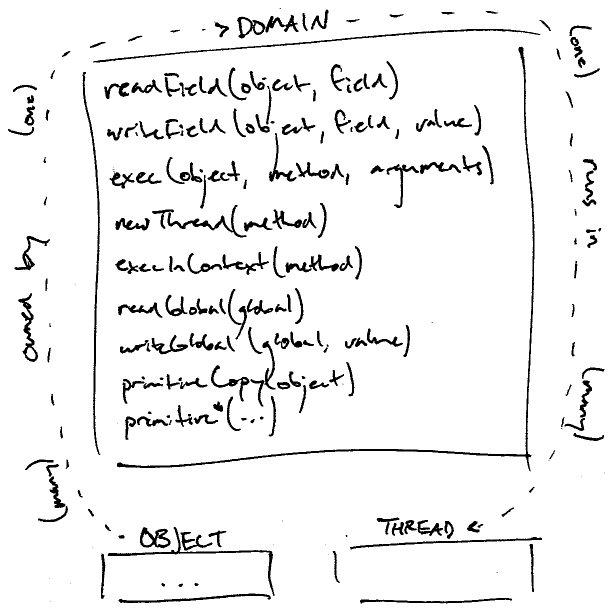
\includegraphics[width=150pt]{obmop}
  \end{frame}

  \section{Conclusion}

  \begin{frame}
    \frametitle{Future work}
  \end{frame}

  \begin{frame}[standout]
    \centering
    Thanks to Elena Machkasova, K.K. Lamberty, and Matthew Justin for their guidance and suggestions.
    \vfill
    \href{https://github.com/dstelljes/senior-sem}{github.com/dstelljes/senior-sem}
    \vfill
    \ccbyncsa{}
  \end{frame}

  \appendix{}

  \begin{frame}[allowframebreaks]
    \frametitle{References}

    \printbibliography{}
  \end{frame}

\end{document}
